\documentclass{beamer}

\usepackage[utf8]{inputenc} % allow utf-8 input
\usepackage[T1]{fontenc}    % use 8-bit T1 fonts
\usepackage[build={quote={<char>}}]{standalone}
\usepackage{tikz}

\usepackage{amsmath}
\usepackage{amssymb}
\usepackage{mathtools}
\usepackage{amstext}
\usepackage{amsthm}
\usepackage{fancyhdr}
\usepackage{siunitx}
\usepackage{physics}

\usepackage{hyperref}


\usepackage{graphicx}
\usepackage{float}
\graphicspath{{figures/}} %Setting the graphicspath
\usepackage{float}
\usepackage{caption}
\usepackage{subcaption}

% To work with inkfigures
\usepackage{import}
\usepackage{pdfpages}
\usepackage{transparent}
\usepackage{xcolor}

\newcommand{\angstrom}{\textup{\AA}}
%\numberwithin{equation}{section}
\renewcommand\thesubsection{\alph{subsection})}
\renewcommand\thesubsubsection{\Roman{subsubsection}}
\newcommand{\s}{\hspace{0.1cm}}

%\usetheme{AnnArbor}
%\usetheme{Antibes}
%\usetheme{Bergen}
%\usetheme{Berkeley}
\usetheme{Berlin}
%\usetheme{Boadilla}
%\usetheme{boxes}
%\usetheme{CambridgeUS}
%\usetheme{Copenhagen}
%\usetheme{Darmstadt}
%\usetheme{default}
%\usetheme{Frankfurt}
%\usetheme{Goettingen}
%\usetheme{Hannover}
%\usetheme{Ilmenau}
%\usetheme{JuanLesPins}
%\usetheme{Luebeck}
%\usetheme{Madrid}
%\usetheme{Malmoe}
%\usetheme{Marburg}
%\usetheme{Montpellier}
%\usetheme{PaloAlto}
%\usetheme{Pittsburgh}
%\usetheme{Rochester}
%\usetheme{Singapore}
%\usetheme{Szeged}
%\usetheme{Warsaw}

\usefonttheme[onlymath]{serif}
% Astronomy
\DeclareSIUnit\parsec{pc}
\DeclareSIUnit\lightyear{ly}


\institute[] % (optional, but mostly needed)
{
		Département de Physique\\
		Université de Montréal
}
\title{Censai}
\subtitle{}

\author{Alexandre Adam}

\date{\today}

\AtBeginSubsection[]
{
  \begin{frame}<beamer>{Résumé}
	\tableofcontents[currentsection,currentsubsection]
  \end{frame}
}

\usepackage[authoryear]{natbib}
\bibliographystyle{abbrvnat}
%\bibliographystyle{apacite}
\captionsetup{labelformat=empty,labelsep=none}



\begin{document}

\begin{frame}
	\titlepage
\end{frame}


\begin{frame}{Recurrent Inference Machine (RIM)}
The RIM is designed to solve problems of the form
\[
	\mathbf{y} = f(\mathbf{x}) + \boldsymbol{\eta} 
\]
The noise model is usually chosen to be Gaussian $\boldsymbol{\eta} \sim \mathcal{N}(0,\, \Sigma) $, such that
\[
	\log\mathcal{L}(\mathbf{y} \mid \mathbf{x}) \propto - \frac{1}{2}(\mathbf{y} - f(\mathbf{x}))^T
\Sigma^{-1}(\mathbf{y} - f(\mathbf{x}))
\]

RIM solves this problem recursively, similarly to a downhill optimizer
\[
	\mathbf{\hat{x}}_{t+1} = \mathbf{\hat{x}}_t + 
\underbrace{
g_\varphi(\mathbf{x}_t, \grad \mathcal{L}_{\mathbf{y} \mid\mathbf{\hat{x}}_t })
}_{-\gamma_t\Delta \mathbf{\hat{x}}_t}
\]
\end{frame}


\begin{frame}{Estimating Background Source Brightness}
        {Morningstar, Perreault-Levasseur \textit{et al.}}
\begin{figure}[H]
        \centering
        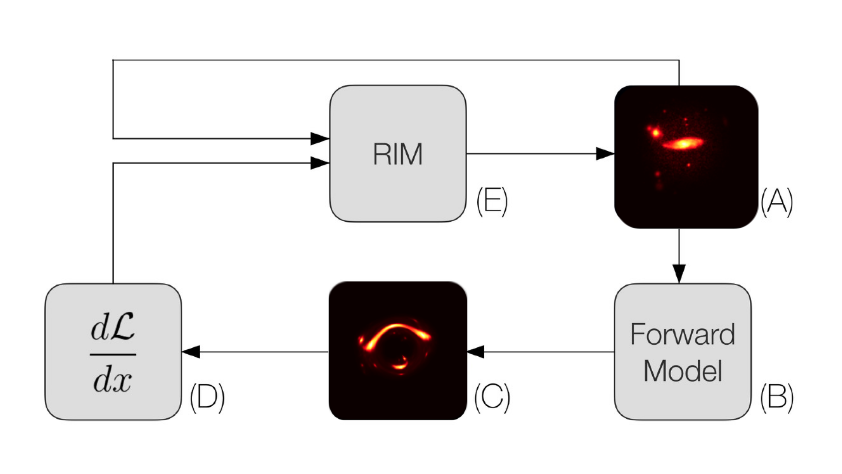
\includegraphics[width=0.8\textwidth]{slide_morningstar2019}
\end{figure}
\end{frame}

\begin{frame}{Estimating both source and $\kappa$}{Adam, Perreault-Levasseur \textit{et al.}, in prep.}
\begin{figure}[H]
        \includestandalone[mode=image,width=0.6\linewidth]{figures/rim2021}
\end{figure}
\end{frame}

%\begin{frame}[plain]{Realistic Mass Distributions}{Illustris TNG 100-1}
%\begin{figure}[H]
        %\centering
        %\includegraphics[keepaspectratio, width=\paperwidth, height=\paperheight]{}
%\end{figure}
%\end{frame}

{ % all template changes are local to this group.
    %\setbeamertemplate{navigation symbols}{}
        \begin{frame}[plain]{Simulated Mass Distributions}{Illustris TNG100-1: Dark Matter, Baryons, Gas and Black Holes}
        \begin{tikzpicture}[remember picture,overlay]
            \node[at=(current page.center)] {
                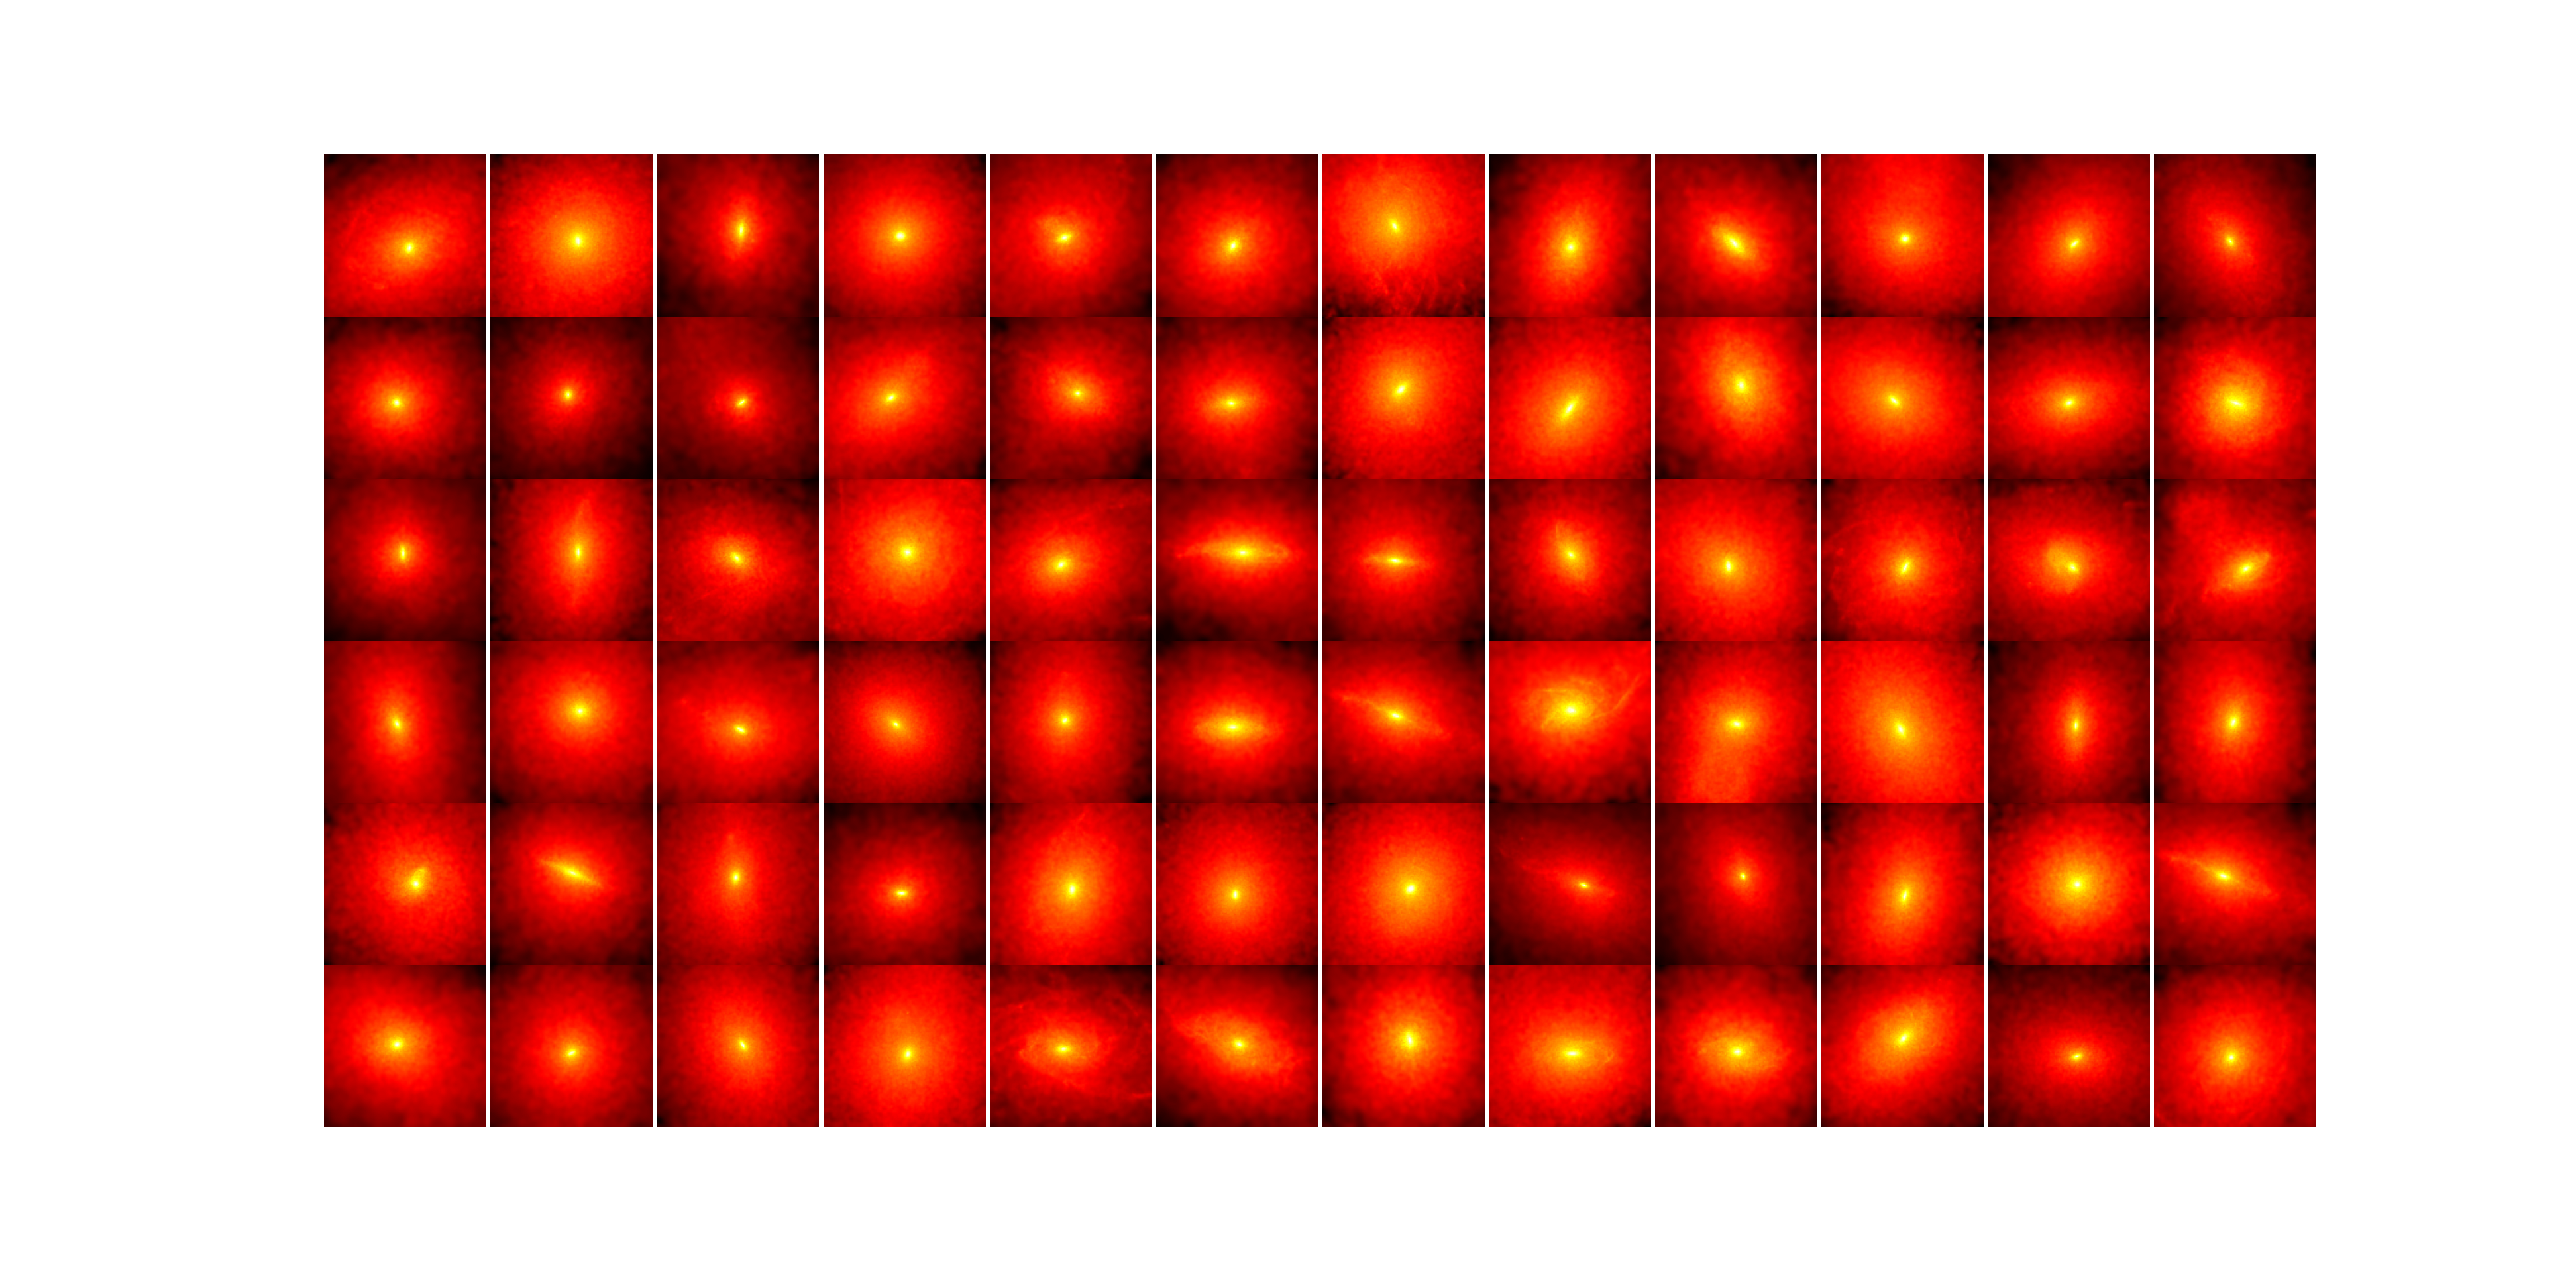
\includegraphics[keepaspectratio,
                            width=1.2\paperwidth,
                        height=1.\paperheight]{figures/KappaTNG100}
            };
        \end{tikzpicture}
     \end{frame}
}

\begin{frame}{Data Augmentation}{VAE}
        \begin{figure}[H]
                \centering
                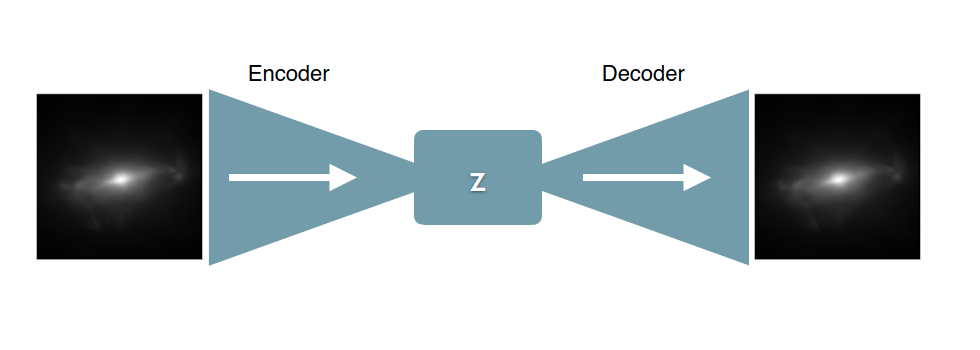
\includegraphics[width=0.8\textwidth]{figures/vae}
        \end{figure}
        
\end{frame}


\begin{frame}{Original Architecture}{}
\begin{figure}[H]
        \includestandalone[mode=image,width=\linewidth]{figures/unet2019}
\end{figure}
\end{frame}

\begin{frame}{New Architecture}{}
\begin{figure}[H]
        \includestandalone[mode=image,width=\linewidth]{figures/unet2}
\caption{}
\label{fig:}
\end{figure}

\end{frame}


\begin{frame}{Early Results}{}
\begin{figure}[H]
        \centering
        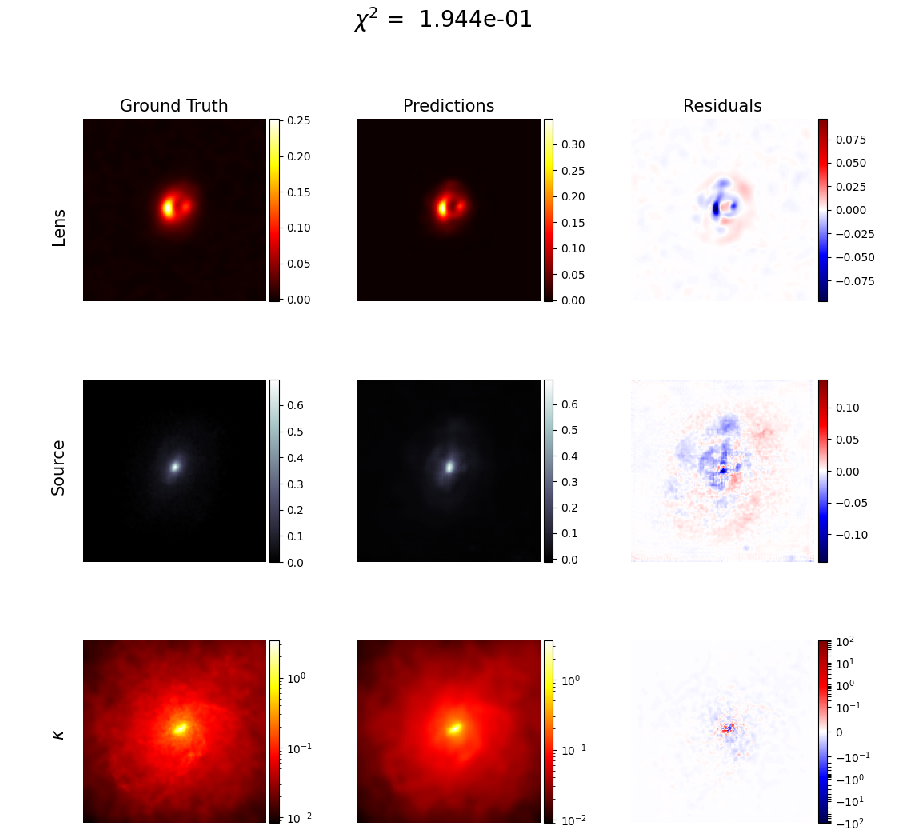
\includegraphics[width=0.65\textwidth]{figures/insane_residual}
        \caption{}
        \label{fig:}
\end{figure}
        

\end{frame}

\end{document}

